\section*{Appendix}

\subsection*{Diagramme}
In diesem Abschnitt werden manche der verwendeten Abbildungen in gr��erer Version aufgef�hrt.

%Kapitel2
\begin{figure}[H]
    \centering
    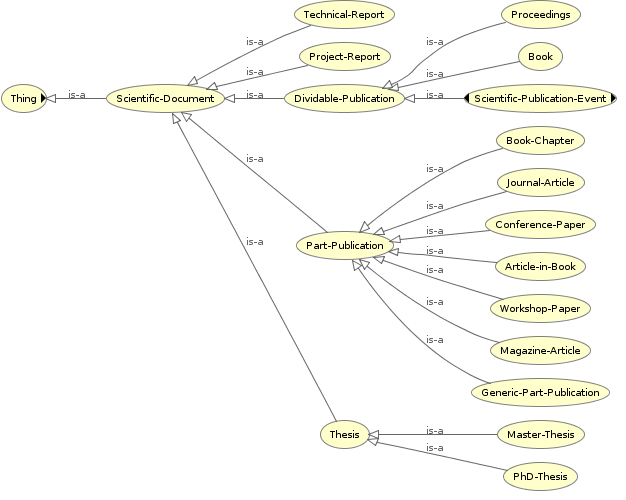
\includegraphics[angle=90,scale=0.65]{../deps/ontology_of_science_scientificdoc_owlviz.png}
    \caption{Ontology of Science. Die Klasse \textit{Scientific Document}}
    \label{fig:scientificdociBig}
\end{figure}

%Kapitel 3
\begin{figure}[H]
        \centering
        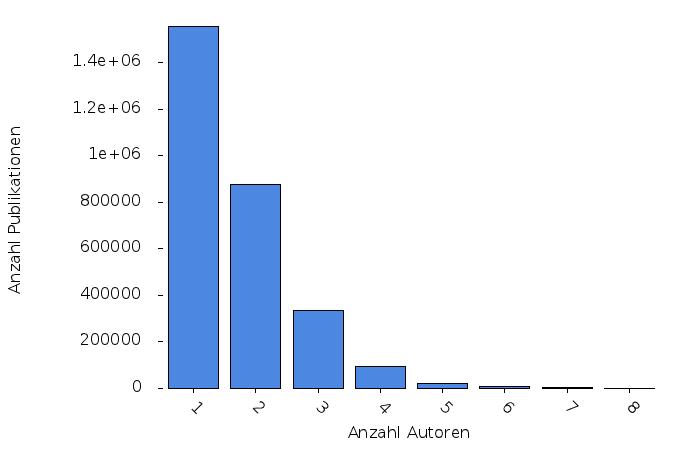
\includegraphics[scale=0.5]{../data/statistics/authorFreq.png}
        \caption{Autorenverteilung}
        \label{fig:authorFreqBig}
\end{figure}

\begin{figure}[H]
        \centering
        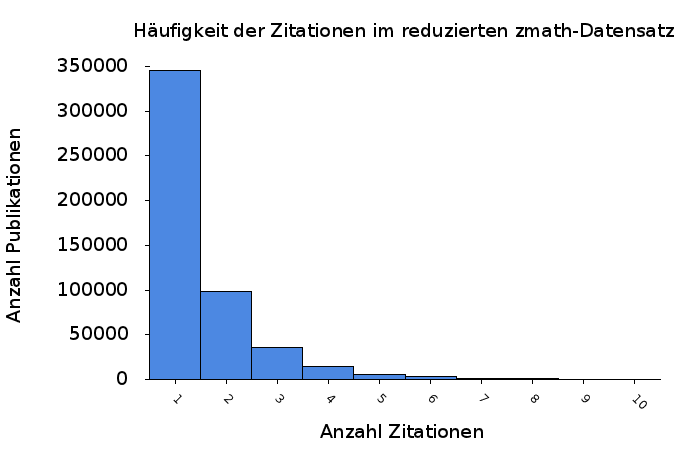
\includegraphics[scale=.5]{../data/statistics/citationFreq.png}
        \caption{Zitationsverteilung}
        \label{fig:citationFreqBig}
\end{figure}

\begin{figure}[H]
        \centering
        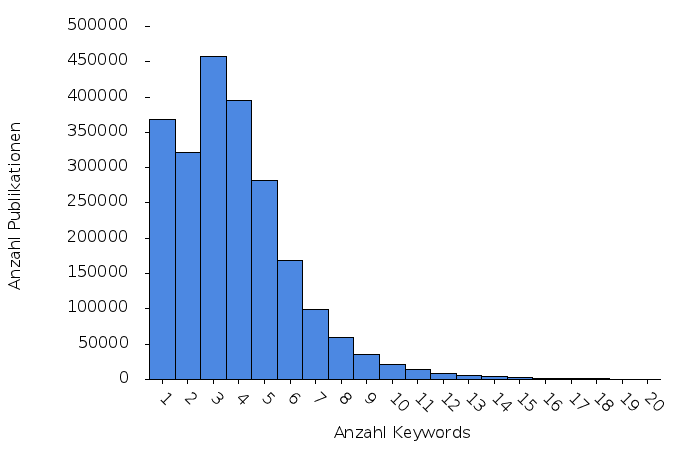
\includegraphics[scale=.5]{../data/statistics/keyWordFreq.png}
        \caption{Keywordverteilung}
        \label{fig:keywordFreqBig}
\end{figure}

\begin{figure}[H]
        \centering
        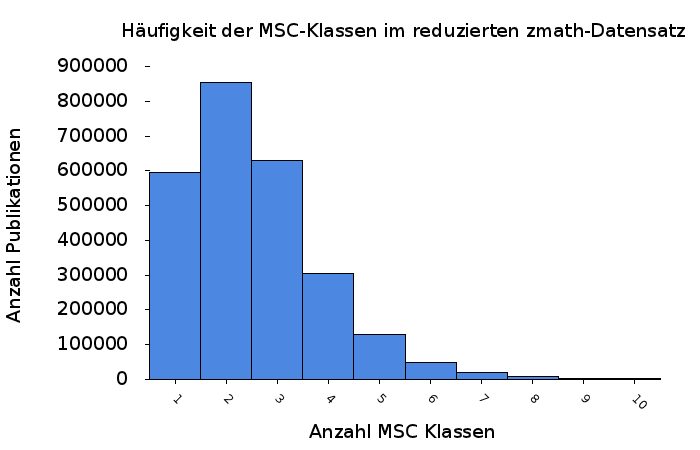
\includegraphics[scale=.5]{../data/statistics/mscClassFreq.png}
        \caption{Verteilung der MSC-Klassen}
        \label{fig:mscClassFreqBig}
\end{figure}

%Kapitel 4
\begin{figure}[H]
        \centering
        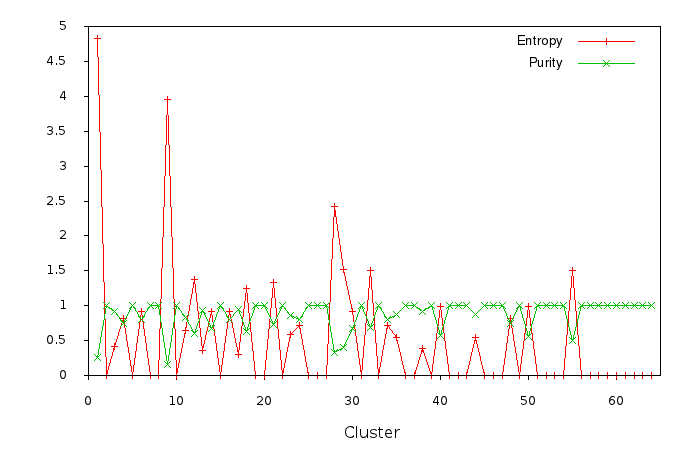
\includegraphics[scale=0.5]{../evaluation/diss_true/crankPurityEntropy.png}
        \caption{Purity und Entropy des \textit{pam}-Clustering von \textit{C-Rank}}
        \label{fig:crankEntPurBig}
\end{figure}


\begin{figure}[H]
        \centering
        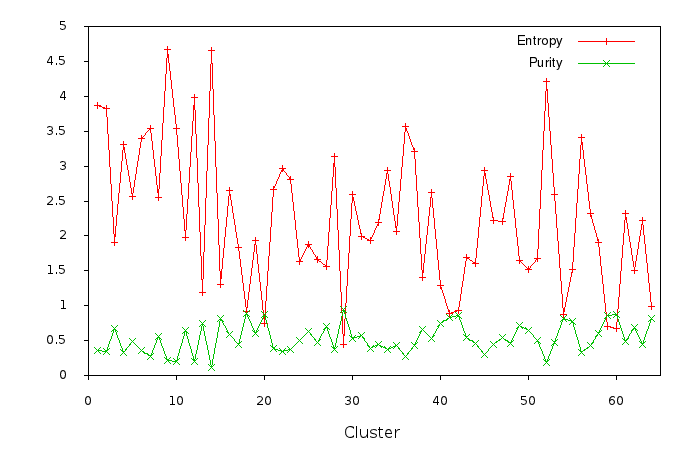
\includegraphics[scale=0.5]{../evaluation/diss_true/p1PurityEntropy.png}
        \caption{Purity und Entropy des \textit{pam}-Clustering von Gewichtung 1}
        \label{fig:p1EntPurBig}
\end{figure}

\begin{figure}[H]
        \centering
        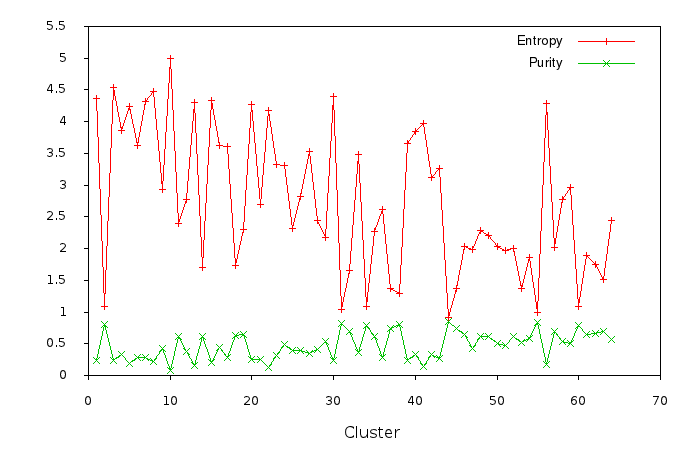
\includegraphics[scale=0.5]{../evaluation/diss_true/p2PurityEntropy.png}
        \caption{Purity und Entropy des \textit{pam}-Clustering von Gewichtung 2}
        \label{fig:p2EntPurBig}
\end{figure}

\begin{figure}[H]
        \centering
        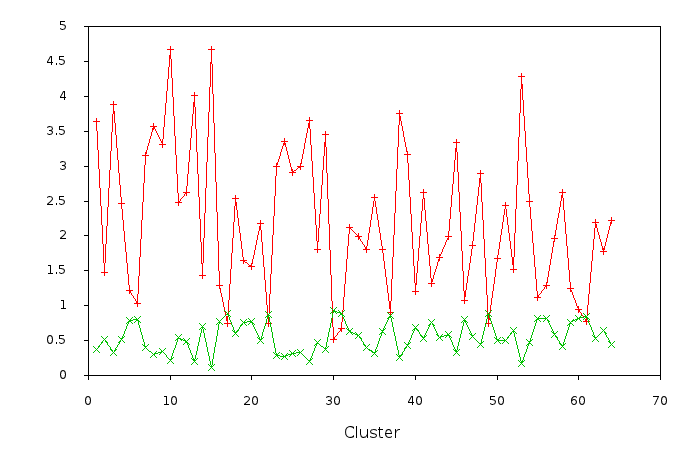
\includegraphics[scale=0.5]{../evaluation/diss_true/p3PurityEntropy.png}
        \caption{Purity und Entropy des \textit{pam}-Clustering von Gewichtung 3}
        \label{fig:p3EntPurBig}
\end{figure}

\subsection*{Ergebnisse des \textit{pam} Clustering}

\begin{longtable}[H]{| l | l | l | l | l |}
%\begin{tabular}{| l | l | l | l | l |}
		\multicolumn{2}{l}{\textbf{C-Rank}} \\
		\hline
        \textbf{ClusterID} & \textbf{\# Publikationen} & \textbf{Entropy} & \textbf{Purity} & \textbf{Gr��te MSC Klasse}\\
	    \hline
        $1$ & $2587$ & $4.8228$ & $0.2613$ & 11-XX : 676 Pubs\\
        $2$ & $10$ & 0 & 1.0 & 11-XX : $10$ Pubs\\
        $3$ & $12$ & 0.413816850304 & 0.916666666667 & 11-XX : $11$ Pubs\\
        $4$ & $4$ & 0.811278124459 & 0.75 & 16-XX : $3$ Pubs\\
        $5$ & $9$ & 0 & 1.0 & 11-XX : $9$ Pubs\\
        $6$ & $10$ & 0.921928094887 & 0.8 & 20-XX : $8$ Pubs\\
        $7$ & $16$ & 0 & 1.0 & 11-XX : $16$ Pubs\\
        $8$ & $16$ & 0 & 1.0 & 11-XX : $16$ Pubs\\
        $9$ & $26$ & 3.95006375644 & 0.153846153846 & 46-XX : $4$ Pubs\\
        $10$ & $9$ & 0 & 1.0 & 47-XX : $9$ Pubs\\
        $11$ & $6$ & 0.650022421648 & 0.833333333333 & 57-XX : $5$ Pubs\\
        $12$ & $5$ & 1.37095059445 & 0.6 & 16-XX : $3$ Pubs\\
        $13$ & $15$ & 0.353359335021 & 0.933333333333 & 11-XX : $14$ Pubs\\
        $14$ & $6$ & 0.918295834054 & 0.666666666667 & 11-XX : $4$ Pubs\\
        $15$ & $15$ & 0 & 1.0 & 11-XX : $15$ Pubs\\
        $16$ & $10$ & 0.921928094887 & 0.8 & 06-XX : $8$ Pubs\\
        $17$ & $19$ & 0.297472248919 & 0.947368421053 & 11-XX : $18$ Pubs\\
        $18$ & $11$ & 1.24067053168 & 0.636363636364 & 76-XX : $7$ Pubs\\
        $19$ & $3$ & 0 & 1.0 & 54-XX : $3$ Pubs\\
        $20$ & $7$ & 0 & 1.0 & 11-XX : $7$ Pubs\\
        $21$ & $22$ & 1.33420945945 & 0.727272727273 & 05-XX : $16$ Pubs\\
        $22$ & $5$ & 0 & 1.0 & 11-XX : $5$ Pubs\\
        $23$ & $7$ & 0.591672778582 & 0.857142857143 & 11-XX : 6.0 Pubs\\
        $24$ & $5$ & 0.721928094887 & 0.8 & 47-XX : $4$  Pubs\\
        $25$ & $13$ & 0 & 1.0 & 11-XX : $13$  Pubs\\
        $26$ & $3$ & 0 & 1.0 & 03-XX : $3$  Pubs\\
        $27$ & $4$ & 0 & 1.0 & 11-XX : $4$  Pubs\\
        $28$ & $12$ & 2.41829583405 & 0.333333333333 & 68-XX : $4$  Pubs\\
        $29$ & $5$ & 1.52192809489 & 0.4 & 91-XX : $2$  Pubs\\
        $30$ & $3$ & 0.918295834054 & 0.666666666667 & 17-XX : $2$  Pubs\\
        $31$ & $4$ & 0 & 1.0 & 62-XX : $4$  Pubs\\
        $32$ & $13$ & 1.5058762556 & 0.692307692308 & 74-XX : $9$  Pubs\\
        $33$ & $6$ & 0 & 1.0 & 11-XX : $6$  Pubs\\
        $34$ & $5$ & 0.721928094887 & 0.8 & 35-XX : $4$  Pubs\\
        $35$ & $8$ & 0.5435644432 & 0.875 & 11-XX : $7$  Pubs\\
        $36$ & $12$ & 0 & 1.0 & 11-XX : $12$  Pubs\\
        $37$ & $7$ & 0 & 1.0 & 11-XX : $7$  Pubs\\
        $38$ & $13$ & 0.391243563629 & 0.923076923077 & 11-XX : $12$  Pubs\\
        $39$ & $14$ & 0 & 1.0 & 11-XX : $14$  Pubs\\
        $40$ & $7$ & 0.985228136034 & 0.571428571429 & 68-XX : $4$  Pubs\\
        $41$ & $8$ & 0 & 1.0 & 11-XX : $8$  Pubs\\
        $42$ & $7$ & 0 & 1.0 & 11-XX : $7$  Pubs\\
        $43$ & $3$ & 0 & 1.0 & 03-XX : $3$  Pubs\\
        $44$ & $8$ & 0.5435644432 & 0.875 & 54-XX : $7$ Pubs\\
        $45$ & $4$ & 0 & 1.0 & 54-XX : $4$  Pubs\\
        $46$ & $6$ & 0 & 1.0 & 54-XX : $6$  Pubs\\
        $47$ & $11$ & 0 & 1.0 & 54-XX : $11$  Pubs\\
        $48$ & $4$ & 0.811278124459 & 0.75 & 26-XX : $3$ Pubs\\
        $49$ & $7$ & 0 & 1.0 & 11-XX : $7$  Pubs\\
        $50$ & $9$ & 0.991076059838 & 0.555555555556 & 11-XX : $5$  Pubs\\
        $51$ & $3$ & 0 & 1.0 & 16-XX : $3$  Pubs\\
        $52$ & $4$ & 0 & 1.0 & 11-XX : $4$  Pubs\\
        $53$ & $6$ & 0 & 1.0 & 11-XX : $6$  Pubs\\
        $54$ & $6$ & 0 & 1.0 & 11-XX : $6$  Pubs\\
        $55$ & $4$ & 1.5 & 0.5 & 49-XX : $2$  Pubs\\
        $56$ & $2$ & 0 & 1.0 & 11-XX : $2$  Pubs\\
        $57$ & $9$ & 0 & 1.0 & 11-XX : $9$  Pubs\\
        $58$ & $8$ & 0 & 1.0 & 53-XX : $8$  Pubs\\
        $59$ & $3$ & 0 & 1.0 & 54-XX : $3$  Pubs\\
        $60$ & $4$ & 0 & 1.0 & 11-XX : $4$  Pubs\\
        $61$ & $4$ & 0 & 1.0 & 11-XX : $4$  Pubs\\
        $62$ & $5$ & 0 & 1.0 & 00-XX : $5$  Pubs\\
        $63$ & $4$ & 0 & 1.0 & 30-XX : $4$  Pubs\\
        $64$ & $2$ & 0 & 1.0 & 11-XX : $2$  Pubs\\
        \hline
%\end{tabular}
\end{longtable}

\subsection*{Berechnung des �hnlichkeitsma�es}
In diesem Appendix wird die erste Iteration, die f�r die Berechnung der semantischen �hnlichkeit erfoderlich ist, f�r zwei Publikationen aus dem \textit{zmath}-Datensatz beispielhaft durchgef�hrt.

\begin{table}[H]
\begin{tabular}{l l}
		%\hline
		\multicolumn{2}{l}{\textbf{Publikation 1}} \\
		%\hline
	    :id: & 3006698 \\
        :an: & 0005.25102\\
        :py: & 1931\\
        :au: & Myrberg, P.J.\\
        :ai: & myrberg.pekka-j\\
        :ti: & �ber beschr�nkte Funktionen in mehrfach zusammenh�ngenden Bereichen.\\
        :so: & Ann. Acad. Sci. Fenn., Ser. A 33, No.8, 1-15 (1931).\\
        :ut: & complex functions\\
        :la: & DE \\
	    %\hline
\end{tabular}
\end{table}

\begin{table}[H]
\begin{tabular}{l p{10cm}}
		%\hline
	    \multicolumn{2}{l}{\textbf{Publikation 2}} \\
		%\hline
	    :id: & 5166522\\
        :an: & 1153.00002\\
        :py: & 2005\\
        :au: & Leonov, Sergey A.; Leonov, Alexander I.\\
        :ai: & leonov.sergey-a; leonov.alexander-i\\
        :ti: & Mathematical handbook for electrical engineers.\\
        :so: & Artech House Technology Management and Professional Development Library. London: Artech House (ISBN 978-1-58053-779-7/hbk). xviii, 495~p. (2005).\\
        :ut: & algebra; functions; equations; combinations; planar and solid geometry; trigonometry; analytic geometry; integral and differential calculus; differential equations; complex functions; Fourier series; vector algebra; probability; applied statistics; computer-aided computation; electrical circuits; antennas; waves; scattering; signal processing; stochastic radio engineering\\
        :la: & EN \\
	    %\hline
\end{tabular}
\end{table}


%::::
%:::
%:id:    5166522
%:an:    1153.00002
%:py:    2005
%:au:    Leonov, Sergey A.; Leonov, Alexander I.
%:ai:    leonov.sergey-a; leonov.alexander-i
%:ti:    Mathematical handbook for electrical engineers.
%:so:    Artech House Technology Management and Professional Development Library. London: Artech House (ISBN 978-1-58053-779-7/hbk). xviii, 495~p. \sterling~85.00 (2005).
%:cc:    00A06 26-00 35-00 60-00 62-00 78-00 94-00
%:ut:    algebra; functions; equations; combinations; planar and solid geometry; trigonometry; analytic geometry; integral and differential calculus; differential equations; complex functions; Fourier series; vector algebra; probability; applied statistics; computer-aided computation; electrical circuits; antennas; waves; scattering; signal processing; stochastic radio engineering
%:la:    EN
%:ci:    
%:li:    


\begin{math}
\begin{array}{lcl}
R_1(P1,P2) & = & 
        \lambda_1\times\cfrac{c}{|K(P1)||K(P2)|}
        \sum_{i=1}^{|K(P1)|} \sum_{j=1}^{|K(P2)|} R_0(K_i(P1),K_j(P2))
        \\ & + &
        \lambda_2\times\cfrac{c}{|A(P1)||A(P2)|}
        \sum_{i=1}^{|A(P1)|} \sum_{j=1}^{|A(P2)|} R_0(A_i(P1),A_j(P2))
        \\ & + &
        \lambda_3\times\cfrac{c}{|S(P1)||S(P2)|}
        \sum_{i=1}^{|S(P1)|} \sum_{j=1}^{|S(P2)|} R_0(S_i(P1),S_j(P2))
        \\ & + &
        \lambda_4\times\cfrac{c}{|C(P1)||C(P2)|}
        \sum_{i=1}^{|C(P1)|} \sum_{j=1}^{|C(P2)|} R_0(C_i(P1),C_j(P2))
        \\ & + &
        \lambda_5\times\cfrac{c}{|Y(P1)||Y(P2)|}
        \sum_{i=1}^{|Y(P1)|} \sum_{j=1}^{|Y(P2)|} R_0(Y_i(P1),Y_j(P2))
        \\ & &
        \\ & = &
        \lambda_1 * \cfrac{c}{1*21} * (R_0(K_1(P1),K_1(P2)) + R_0(K_1(P1),K_2(P2))+
        \\ & &
        \\ & & ... + R_0(K_1(P1),K_{21}(P2)))
        \\ & + &
        \lambda_2 * \cfrac{c}{1*2} * (R_0(A_1(P1),A_1(P2)) + R_0(A_1(P1),A_2(P2)))
        \\ & + &
        \lambda_3 * \cfrac{c}{1*1} * R_0(S_1(P1),S_1(P2))
        \\ & + &
        0
        \\ & + &
        \lambda_5 * \cfrac{c}{1*1} * R_0(Y_1(P1),Y_1(P2))
        \\ & = &
        \lambda_1 * \cfrac{c}{1*21}*(0 + 0 +... +0 + 1 + 0 + ..+ 0)
        \\ & + &
        \lambda_2 * \cfrac{c}{1*2} * (0 + 0)
        \\ & + &
        \lambda_3 * \cfrac{c}{1*1} * 0
        \\ & + &
        0
        \\ & + &
        \lambda_5 * \cfrac{c}{1*1} * 0
        \\ & = &
        \lambda_1 * \cfrac{c}{21} * 1


\end{array}
\end{math}

\bigskip
Dieser erste Iterationsschritt wird auch f�r alle Kombinationen aus jeweils zwei Keywords, zwei Autoren, zwei Quellen und zwei Erscheinungsjahre ausgef�hrt.
F�r jedes Paare derselben Klasse (z.B. zwei Keywords) wird die �hnlichkeit nach der folgenden Formel bestimmt.
Dabei sind L(a) die Publikationen, die das Keyword $a$ verwenden.
Es kann hier leider kein wahrheitsgetreuer Iterationsschritt f�r Keywords beispielhaft vorgef�hrt werden, da wir daf�r alle Publikationen im Datensatz, die diese Keywords verwenden, raussuchen sollten.
Ein Anfang der �hnlichkeitsberechnung f�r die Keywords \textit{complex functions} und \textit{Fourier series} wird folgenderma�en aussehen.
\medskip

\begin{math}
\begin{array}{lcl}
R_1(a,b) &  = &
        \cfrac{c}{|L(a)||L(b)|} *
        \sum_{i=1}^{|L(a)|} \sum_{j=1}^{|L(b)|} R_0(L_i(a),L_j(b))
        \\ & = &
        \cfrac{c}{|L(a)||L(b)|} * (R_0(L_1(a), L_1(b)) + R_0(L_1(a),L_2(b)) + ... + R_0(L_n(a),L_m(b)))
        \\ & = &
        \cfrac{c}{|L(a)||L(b)|} * (... + R_0(P2,P2) + ..)
        \\ & = &
        \cfrac{c}{|L(a)||L(b)|} * (... + 1 + ..)

\end{array}
\end{math}


\bigskip
Bei dem zweiten Iterationsschritt werden dann die Werte aus dem Ersten eingesetzt.
$R_2$ wird aufgrund von $R_1$ berechnet.
